\documentclass[a4paper,12pt]{article}
\usepackage[utf8]{inputenc}
\usepackage{graphicx}
\usepackage{geometry}
\geometry{margin=2cm}
\usepackage{graphicx} % Required for inserting images

\title{La cellula, molecole ed organuli}
\author{Orcam}
\date{}

\begin{document}

\maketitle

\section*{Cellula animale eucariotica}
La cellula è la più piccola unità strutturale e funzionale capace di svolgere i processi vitali. Le attività funzionali dipendono dalle proprietà strutturali specifiche, e tutte le nuove cellule si originano da cellule pre-esistenti.

\subsection*{Principi della teoria cellulare}

    
- Le cellule sono le unità costitutive viventi di tutti gli organismi.
    
- La struttura e la funzione di un organismo dipendono dai loro costituenti cellulari.


\subsection*{Macromolecole biologiche}
Le macromolecole fondamentali sono:

    
- \textbf{Proteine}: Polimeri di aminoacidi (20 tipi, di cui 8 essenziali). Funzioni: enzimi, trasportatori, segnalazione, recettori, regolazione, immunoglobuline.
    
- \textbf{Carboidrati}: Fonte di energia (glucosio) e riserva (glicogeno).
    
- \textbf{Lipidi}: Molecole non polari; costituenti fondamentali delle membrane cellulari.
    
- \textbf{Nucleotidi}: Fondamentali per il trasferimento di energia (ATP) e informazione genetica (DNA, RNA).


\subsection*{Compartimenti principali della cellula}
\begin{enumerate}
    \item \textbf{Membrana plasmatica}: Regola il traffico di materiali.
    \item \textbf{Nucleo}: Contiene il DNA organizzato in cromosomi, associato a proteine istoniche. Controlla la sintesi di mRNA, rRNA e tRNA.
    \item \textbf{Citoplasma}: Contiene organelli come ribosomi, reticolo endoplasmatico (rugoso e liscio), apparato di Golgi, lisosomi, perossisomi e mitocondri.
\end{enumerate}

\subsection*{Organelli cellulari}

    
- \textbf{Reticolo endoplasmatico rugoso (RER)}: Sede della sintesi proteica.
    
- \textbf{Reticolo endoplasmatico liscio (REL)}: Implicato nella maturazione delle proteine e detossificazione.
    
- \textbf{Apparato di Golgi}: Modifica, imballa e distribuisce proteine e lipidi.
    
- \textbf{Lisosomi}: Degradano detriti cellulari e materiali esogeni.
    
- \textbf{Perossisomi}: Contengono enzimi ossidativi e catalasi per la detossificazione.
    
- \textbf{Mitocondri}: Producono energia attraverso la respirazione cellulare. Contengono DNA mitocondriale e ribosomi propri.


\subsection*{Via metabolica cellulare}

    
- \textbf{Aerobica}: Richiede ossigeno, avviene nei mitocondri.
    
- \textbf{Anaerobica}: Non richiede ossigeno, mitocondri non necessari.


\subsection*{Fonte di energia cellulare}
L'energia deriva dalla scissione dei legami carbonio-idrogeno delle sostanze nutritive. Viene immagazzinata sotto forma di ATP e NADH, utilizzate nelle reazioni chimiche cellulari.

% Inserisci qui le immagini
\subsection*{Immagini}
\begin{figure}[h!]
    \centering
    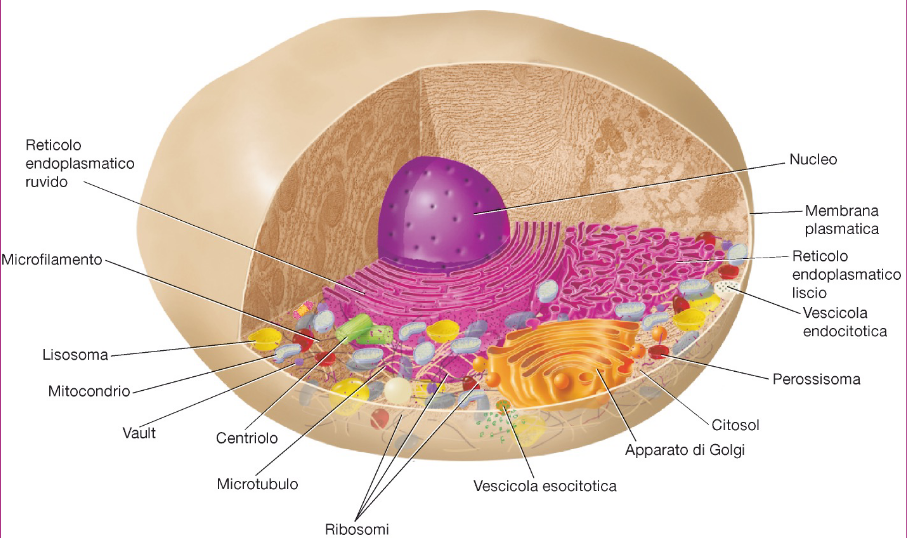
\includegraphics[width=0.8\textwidth]{Neuroscienze 2024-2025/Modulo I/Screenshot 2025-06-20 at 15-31-51 2. La cellula molecole ed organuli.pdf.png} % Sostituisci con il nome del file dell'immagine
    \caption{Struttura della cellula eucariotica.}
\end{figure}

\begin{figure}[h!]
    \centering
    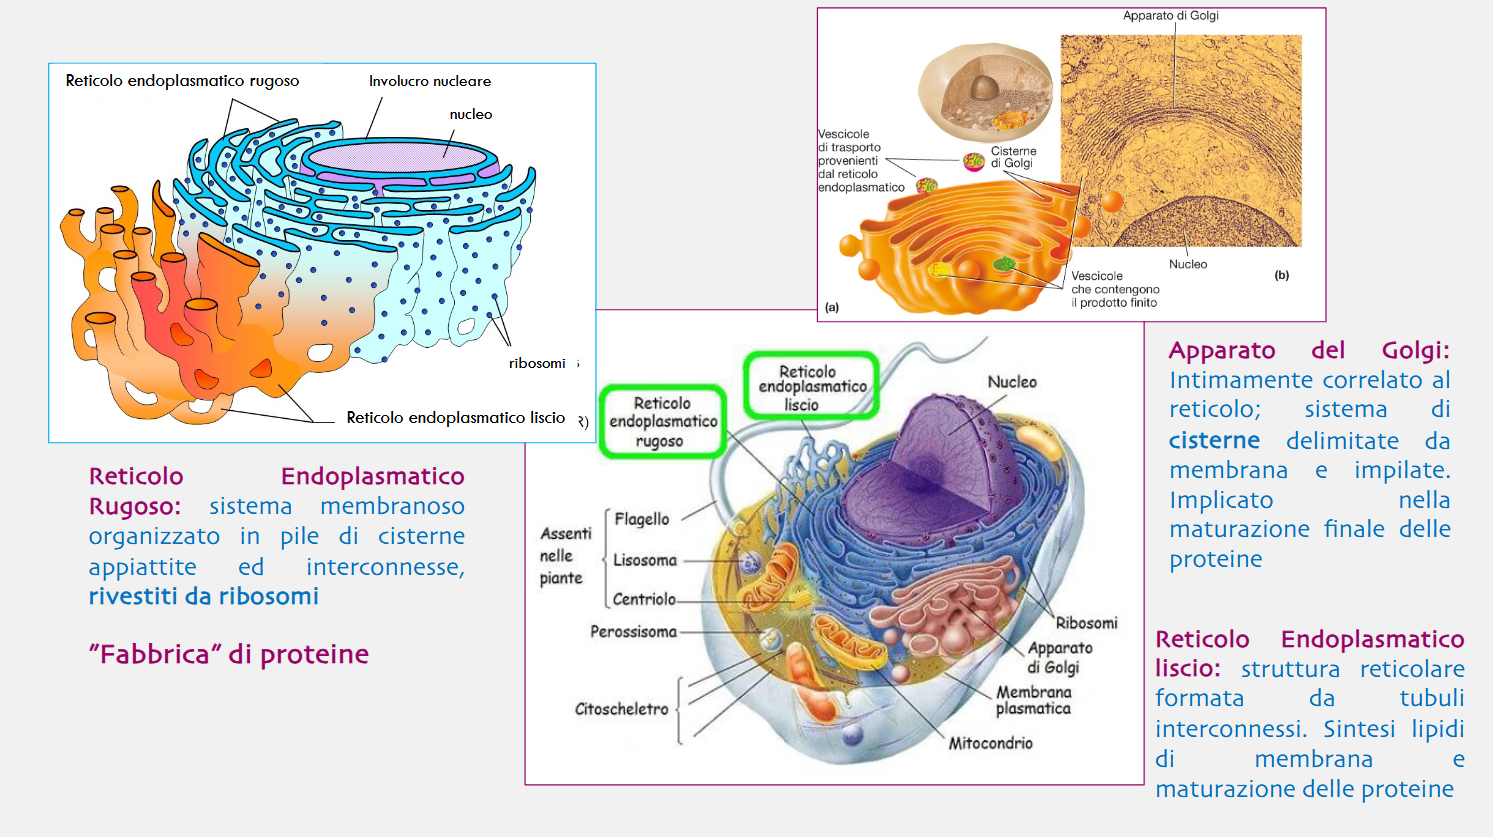
\includegraphics[width=1\textwidth]{Neuroscienze 2024-2025/Modulo I/Screenshot 2025-06-20 at 15-32-28 2. La cellula molecole ed organuli.pdf.png} % Sostituisci con il nome del file dell'immagine
    \caption{Dettaglio degli organelli cellulari.}
\end{figure}

\end{document}

\end{document}

